% TODO:

% Write ``Liquid-vapor interface'' section A.

% Look up question-mark references (citations).

\documentclass[letterpaper,twocolumn,amsmath,amssymb,jcp,10pt,aip]{revtex4-1}
\usepackage{graphicx}% Include figure files
\usepackage{dcolumn}% Align table columns on decimal point
\usepackage{bm}% bold math
\usepackage{color}

\newcommand{\red}[1]{{\bf \color{red} #1}}
\newcommand{\blue}[1]{{\bf \color{blue} #1}}
\newcommand{\green}[1]{{\bf \color{green} #1}}
\newcommand{\rr}{\textbf{r}}
\newcommand{\refnote}{\red{[ref]}}

\newcommand{\fixme}[1]{\red{[#1]}}

%\newcommand{\derivation}[1]{#1} % Use this to show all derivations in detail
\newcommand{\derivation}[1]{} % Use this for nice pegagogical paper...

% needsworklater is used to annotate bits that need work, but that we
% can postpone for a while.
\newcommand{\needsworklater}[1]{\emph{[#1]}}
% needsworknow is intended to prioritize stuff that needs fixing.
\newcommand{\needsworknow}[1]{\textcolor{red}{[\emph{#1}]}}

\begin{document}
\title{Using Fundamental Measure Theory to Treat the Correlation
  Function of the Inhomogeneous Hard-Sphere Fluid}

\author{Jeff Schulte}
\author{Patrick Kreitzburg}
\author{Chris Haglund}
\author{David Roundy}
\affiliation{Department of Physics, Oregon State University, Corvallis, OR 97331}


%%%%%%%%%%%%%%%%%%%%%%%%%%%%%%%%%%%%%%%%%%%%%%%%%%%%%%%%%%%%
\begin{abstract}
  We investigate the value of the correlation function an
  inhomogeneous hard-sphere fluid at contact $g_\sigma$.  This
  quantity plays a critical role in Statistical Associating Fluid
  Theory (SAFT), which is the basis of a number of recent classical
  density functionals.  We define two averaged values for the
  correlation function at contact, and derive formulas for each of
  them from the White Bear version of the Fundamental Measure Theory
  functional~\cite{roth2002whitebear}, based on an assumption of
  thermodynamic consistency. We have tested these functionals and two
  existing functionals~\cite{yu2002fmt-dft-inhomogeneous-associating,
    gross2009density} against Monte Carlo simulations.  We find
  excellent agreement between the Monte Carlo data and our
  asymmetrically averaged correlation function, and less impressive
  agreement with the other three correlation functionals.
\end{abstract}

\maketitle

%%%%%%%%%%%%%%%%%%%%%%%%%%%%%%%%%%%%%%%%%%%%%%%%%%%%%%%%%%%%
\section{Introduction}

% The following are papers that use a SAFT-based classical DFT with at
% least some of the terms purely local
\newcommand\saftlocaldft{felipe2001examination, gloor2002saft,%
  gloor2004accurate, clark2006developing, gloor2007prediction,%
  kahl2008modified, gross2009density}
% The following are papers that use a SAFT-based classical DFT with
% all the terms that should be non-local being non-local.
\newcommand\saftnonlocaldft{yu2002fmt-dft-inhomogeneous-associating,%
  fu2005vapor-liquid-dft,bryk2006density}

There has been considerable recent interest in using Statistical
Associating Fluid Theory (SAFT) to construct classical density
functionals to describe associating
fluids\cite{\saftlocaldft,\saftnonlocaldft}.  This approach has been
successful in qualitatively describing the dependence of surface
tension on temperature.
%
%% Unfortunately, most of these constructed
%% functionals\cite{\saftlocaldft} cannot be used to study arbitrary
%% inhomogeneous density distributions, because they use local density
%% approximations that are only valid for densities that vary slowly over
%% molecular length scales.
%
A key input to SAFT-based functionals is the correlation function
evaluated at contact.  Although two recent works have introduced
approximate functionals for this
quantity\cite{yu2002fmt-dft-inhomogeneous-associating,
  gross2009density}, there has yet to be a careful study of the
correlation function at contact in the inhomogeneous hard-sphere
fluid.

Constructing a classical density functional based on SAFT involves
rewriting each term in the free energy as a functional of an
inhomogeneous density.  The SAFT free energy consists of four terms:
\begin{align}
  A_\textit{SAFT} &= A_\textit{ideal} + A_\textit{HS} + A_\textit{chain} + A_\textit{disp} + A_\textit{assoc}
\end{align}
where $A_\textit{ideal}$ is the ideal-gas free energy, $A_\textit{HS}$
is the excess free energy of a hard-sphere fluid, $A_\textit{chain}$
is the free energy of formation for polymeric fluids,
$A_\textit{disp}$ is the dispersion contribution to the free energy,
and $A_\textit{assoc}$ is the free energy contribution from
\emph{association}, which is to say, hydrogen bonding.  The chain and
association contributions to the SAFT free energy are of particular
interest for this paper, since each requires as input the contact
value of the correlation function.
%
Yu and Wu introduced in 2002 a functional for the association term of
the free energy, which included a functional for the contact value of
the correlation function (see
Section~\ref{sec:yuwu})\cite{yu2002fmt-dft-inhomogeneous-associating},
which has subsequently been used in the development of other
SAFT-based functionals\cite{fu2005vapor-liquid-dft, bryk2006density}.
%% Each of these terms has some dependence on the
%% inhomogeneity in the density.  The ideal gas is purely local, and in
%% fact must be the only purely local term in the free energy in order
%% for the functional to satisfy the contact-value theorem.  The
%% hard-sphere contribution contribution to the free energy has been
%% thoroughly studied, and is well approximated by the White Bear version
%% of the Fundamental-Measure Theory (FMT)
%% functional\cite{roth2002whitebear}.
Two functionals for the chain contribution have recently been
introduced\cite{bryk2006density, gross2009density}, one which uses the
contact value of the correlation function of Yu and
Wu\cite{bryk2006density}, while the other introduces a new functional
for the contact value of the correlation
function (see Section~\ref{sec:gross})\cite{gross2009density}.
%% The dispersion term is long-range and thus has significant
%% dependence on the density distribution, but because its relatively
%% weak position dependence, is amenable to mean-field approximations.
Given these different approaches, it seems valuable to examine this
property of the hard-sphere fluid through direct simulation, in order
to establish the advantages and disadvantages of each approach.

In this paper we introduce two definitions for the locally averaged
correlation function of an inhomogeneous system.  The first is more
symmetric (which we call the $S$ case), while the second involves a
sphere-centered, assymetrical interpretation (the $A$ case).  Given
these definitions, we will present a thermodynamic approach for
evaluating these these correlation functions directly from the free
energy functional itself.  We will then explain how the correlation
function of Yu and Wu and that of Gross compare with our
definitions---the former is a variant of the $S$ correlation function,
while the latter is an $A$ function.  Finally, we will compare these
four approximations with exact Monte-Carlo simulations for the
hard-sphere fluid in at a variety of hard-wall surfaces.


\section{Correlation function with inhomogeneity}

We will define our terms by making use of the two-particle density
$n^{(2)}(\rr_1,\rr_2)$, which gives the probability per unit volume
squared of finding one particle at position $\rr_1$ and the other at
position $\rr_2$.  The pair correlation function is defined by
\begin{align}
  g(\rr_1,\rr_2) &\equiv \frac{n^{(2)}(\rr_1,\rr_2)}{n(\rr_1)n(\rr_2)}
\end{align}
In a homogeneous fluid, the pair correlation only depends on the
distance $|\rr_1-\rr_2|$, and can be expressed as a function of a
single variable, with the contact value being when that distance is
the diameter $\sigma$.  It is desirable for reasons of efficiency to limit CDFT
functionals to one-center convolutions, which leads us to seek a
simplified expression for the contact value of the correlation
function---which is the same as the contact value of the cavity
correlation function for hard spheres.
In a system with an inhomogeneous density, we seek a \emph{local}
value for $g_\sigma$.  There are two reasonable options for defining
such a local function: a symmetric formulation (which we refer to as $S$) and an
asymmetric formulation (which we refer to as $A$).

For the symmetric $S$ case, the correlation function at contact is
given by:
\begin{align}
  g^S_\sigma(\rr) &= \frac{1}{n_0(\rr)^2}\int n^{(2)}(\rr - \rr', \rr
  + \rr')
  \frac{\delta(|\rr'| -\sigma/2)}{\pi\sigma^2}d\rr' \label{eq:gS}
\end{align}
where density $n_0$ is one of the fundamental measures of Fundamental
Measure Theory (FMT), and is ideal for treating touching spheres, as
illustrated in Figure~\ref{fig:n0}.
\begin{align}
  n_0(\rr) &= \int n(\rr')\frac{\delta(|\rr-\rr'|-\sigma/2)}{\pi\sigma^2} d\rr'
\end{align}
This functional gives a value averaged over all spheres that touch at
the position $\rr$.

\begin{figure}
\includegraphics[width=5cm]{figs/n0}
\caption{Set of hard spheres that included in $n_0(\mathbf{r})$, which
  consist of those which just touch the point $\mathbf{r}$.}
\label{fig:n0}
\end{figure}

In contrast, the asymmetrically averaged $A$ correlation function is
given by
\begin{align}
  g^A_\sigma(\rr) &= \frac{1}{n(\rr)n_A(\rr)}
  \int n^{(2)}(\rr, \rr + \rr')
  \frac{\delta(|\rr'| - \sigma)}{4\pi\sigma^2}d\rr' \label{eq:gA}
\end{align}
where the density $n_A(\rr)$ is similar to $n_0$, but measures the
density of spheres that could be touching a sphere that is located at
point $\rr$.
\begin{align}
  n_A(\rr) &= \int n(\rr')
  \frac{\delta(|\rr-\rr'|-\sigma)}{4\pi\sigma^2} d\rr' \label{eq:nA}
\end{align}
Thus $g_\sigma^A$ corresponds to an average of the two-particle
density over spheres touching a sphere that is located at the
position~$\rr$.

%% In the process of defining these two averaged correlation functions,
%% we also defined two averaged densities, $n_0(\rr)$ and $n_A(\rr)$,
%% which are the density of spheres available to be in
%% contact.  In the homogeneous limit, $n_0 = n_A = n$.  It is an
%% open question, which of these averages will be more useful in any
%% particular functional.  Suffice to say, either average is a
%% \emph{possible} way to convert a function that is defined for a
%% homogeneous system to a functional that is applicable to inhomogeneous
%% systems.

%% Yu and Wu introduce an approximation for
%% $g^S$\cite{yu2002fmt-dft-inhomogeneous-associating}, which we will
%% discus in Section~\ref{sec:yuwu}.  Gross introduced an
%% approximation for $g^A$\cite{gross2009density}, which we will
%% introduce in Section~\ref{sec:gross}.  We will also introduce our own
%% approximations for both $g^A$ and $g^S$ which are based on the
%% assumption of thermodynamic consistency within FMT, in
%% Sections~\ref{sec:g-S} and~\ref{sec:g-A}.  We will report on the accuracy of
%% these approximations by comparing with Monte Carlo simulations of the
%% inhomogeneous hard-sphere fluid.  We will focus on the contact
%% densities, rather than the correlation function itself, because these
%% are simpler, and because they are the quantity that you want to
%% ``average''.  i.e. if you were to average $g$ itself, you'd want to
%% weight that average based on the density, which would mean averaging
%% $n^{(2)}$.


%% \subsection{Association free energy of SAFT}

%% \fixme{Integrate the following equations into this section...}
%% \begin{align}
%%   \frac{A_\textit{chain}}{kT} &= -(m-1) n \left(\ln\left(n g_\sigma \right)-1\right)
%% \end{align}
%% \begin{align}
%%   \frac{A_\textit{assoc}}{kT} &= \sum_i n \left(\ln X_i - \frac12 X_i + \frac12\right) \\
%%   X_i &= \frac{1}{1 + \sum_j n g_\sigma X_j\kappa_{ij} \left(e^{\beta \epsilon_{ij}}-1\right)}
%% \end{align}

%% \newcommand\epsilonassoc{\ensuremath{\varepsilon_\textit{AB}}}
%% \newcommand\kappaassoc{\ensuremath{\kappa_\textit{AB}}}
\newcommand\ncontact{\ensuremath{n_\textit{contact}}}

%% The free energy term in Statistical Associating Fluid Teory (SAFT)
%% from which it derives its name is the association term, which accounts
%% for hydrogen bonding.  Hydrogen bonds are modeled as attractive
%% patches (``association sites'') on the surface of hard spheres.  These
%% sites represent protons or electron lone pairs, and have an attractive
%% energy $\epsilonassoc$ when two molecules are oriented such that the
%% proton of one overlaps with the lone pair of the other.  The volume
%% over which this interaction occurs is $\kappaassoc$, giving the
%% association term in the free energy has two empirical parameters fit
%% to experimental data.

%% The association free energy per unit volume has the form
%% \begin{align}
%%   f_\text{assoc} &= k_BT n\sum_A 
%%                   \left(\ln X^A - \frac{X^A}{2} + \frac12\right)
%% \end{align}
%% where the summation is over the association sites, and $X^A$ is the
%% fraction of association sites \emph{not} hydrogen-bonded.  The
%% fractions $X^A$ are determined by the self-consistent equations
%% \begin{align}
%%   X^A &= \frac{1}
%%   {1 + \sum_B n X^B \Delta^{AB}}\label{eq:X}
%%   \\
%%   \Delta^{AB} &= g(\sigma) \kappaassoc\left( e^{\epsilonassoc/kT} -
%%   1 \right)\label{eq:delta}
%% \end{align}
%% where $g(\sigma)$ is the correlation function evaluated at contact.
%% The product of density with correlation function evaluated at contact
%% gives the contact density, when we combine Equations~\ref{eq:X} and
%% \ref{eq:delta}:
%% \begin{align}
%%   X^A &= \frac{1}
%%   {1 + \sum_B \ncontact\kappaassoc X^B\left( e^{\epsilonassoc/kT} -
%%   1 \right)}
%% \end{align}
%% where the product $\ncontact\kappaassoc$ is the expected number of
%% molecules present in the association volume in the absence of the
%% association interaction.  In the SAFT-VR
%% model\cite{gil-villegas-1997-SAFT-VR}, this contact density is found
%% by adding a perturbative correction to the contact value for a hard
%% sphere fluid.

\subsection{Fundamental-Measure Theory}

We use the White Bear version of the Fundamental-Measure Theory~(FMT)
functional published in reference~\cite{roth2002whitebear}.  The FMT
functional describes the excess free energy of a hard-sphere fluid.
This particular FMT reduces to the Carnahan-Starling equation of state
for homogeneous systems.
\begin{equation}
A_\textit{HS}[n] = k_B T \int \left(\Phi_1(\rr) + \Phi_2(\rr) + \Phi_3(\rr)\right) d\rr \; ,
\end{equation}
with integrands
\begin{align}
\Phi_1 &= -n_0 \ln\left( 1 - n_3\right)\\
\Phi_2 &= \frac{n_1 n_2 - \mathbf{n}_{V1} \cdot\mathbf{n}_{V2}}{1-n_3} \\
\Phi_3 &= (n_2^3 - 3 n_2 \mathbf{n}_{V2} \cdot \mathbf{n}_{V2}) \frac{
  n_3 + (1-n_3)^2 \ln(1-n_3)
}{
  36\pi n_3^2\left( 1 - n_3 \right)^2
} ,
\end{align}
using the weighted densities
\begin{align}
  n_3(\rr) &= \int n(\rr') \Theta(\left|\rr - \rr'\right| - \sigma/2)
  d\rr' \label{eq:FMn3} \\
  n_2(\rr) &= \int n(\rr') \delta(\left|\rr - \rr'\right| - \sigma/2) d\rr' \\
  \mathbf{n}_{2V}(\rr) &= \int n(\rr') \delta(\left|\rr - \rr'\right| - \sigma/2) \frac{\rr-\rr'}{|\rr-\rr'|}d\rr'
\end{align}
\begin{align}
  \mathbf{n}_{V1} = \frac{\mathbf{n}_{V2}}{2\pi \sigma}, \quad
  n_1 &= \frac{n_2}{2\pi \sigma} , \quad
  n_0 = \frac{n_2}{\pi \sigma^2} \label{eq:FMrest}
\end{align}


\section{Theoretical Approaches}

\subsection{Homogeneous limit}

In order to motivate the derivation of our functional for the value of
the correlation function at contact, we begin by deriving the
well-known value of $g_\sigma$ for a homogeneous hard-sphere fluid
from the Carnahan-Starling free energy.  The contact value of the
correlation function density is most easily found by using the
contact-value theorem, which states that the pressure on any hard
surface is determined by the density at contact:
\begin{align}
  p &= k_BT n_\textit{contact} \\
  &= k_BT n g_\sigma
\end{align}
Since we are interested in the correlation function at the surface of
the hard spheres, all we need compute is the pressure on that surface,
and we'll have our answer.  The pressure on a hard sphere can be
readily computed from the dependence of the Carnahan-Starling free
energy on hard sphere radius.
\begin{align}
  A_{HS} &= Nk_BT \frac{4\eta - 3\eta^2}{(1-\eta)^2}
\end{align}
where $\eta \equiv \frac{\pi}{6} \sigma^3 n$ is the filling fraction.  We
can thus readily compute the derivative of free energy with respect to
hard-sphere diameter:
\begin{align}
  \frac{dA_{HS}}{d\sigma} &= \frac{dA_{HS}}{d\eta} \frac{d\eta}{d\sigma} \\
  &= Nk_BT \frac{4 - 2\eta}{(1-\eta)^3} \frac{3 \eta}{\sigma} \label{eq:dAhsdR}
\end{align}
This derivative gives us half the force on \emph{all} the hard
spheres---since we're changing all their radii at once.  To compute
the pressure on the spheres, we just need to divide by half the total
area, which means dividing by $N 8\pi \sigma^2$, since the relevant
area is the area over which the molecules can make contact.
\begin{align}
  p_{HS} &= \frac{1}{N 8\pi \sigma^2} \frac{dA_{HS}}{d\sigma} \\
  &= k_BT n \frac{1 - \frac{\eta}2}{(1-\eta)^3}
\end{align}
Using the contact-value theorem, we can thus find the well-known
correlation function evaluated at contact.
\begin{align}
  g_{HS}(\sigma) &= \frac{1 - \frac{\eta}2}{(1-\eta)^3} \label{eq:cs-g}
\end{align}
Thus we can readily derive the contact density for the homogeneous
hard-sphere fluid.  Extending this derivation to the inhomogeneous
fluid requires that we find the pressure on particular spheres---or
potentially particular parts of particular spheres.


\subsection{Asymmetrically averaged correlation function}\label{sec:g-A}

We will begin our derivation of the locally averaged correlation
function with the asymmetric definition of $g_\sigma^A(\rr)$ given in
Equation~\ref{eq:gA}, which is averaged over contacts in which one of
the two spheres is located at position~$\rr$.  This correlation
function is related to the contact density averaged over the surface
of a sphere located at $\rr$, and can thus be determined by finding
the pressure on that sphere.  We find this pressure by treating the
hard-sphere diameter as a function of the location of the sphere in
question, when defining the fundamental measured (in
Equations~\ref{eq:FMn3}-\ref{eq:FMrest}):
\begin{align}
  n_3^A(\rr) &= \int n(\rr')\Theta(|\rr-\rr'|-\sigma(\rr')/2)d\rr' \label{eq:n3A}
\end{align}
Once we have done this, we derive a formula for the correlation
function $g_\sigma^A(\rr)$ by finding the pressure on the surface of
any hard spheres located at position $\rr$, and using the
contact-density theorem to extract the contact density, from which we
can establish the averaged correlation function at contact.
\begin{align}
  p_{HS}(\mathbf{r}) &= \frac{1}{n(\rr) 2\pi \sigma^2} \frac{\delta
    A_{HS}}{\delta \sigma(\mathbf{r})} \label{eq:p_{HS}^A}\\
%  \ncontact(\rr) &= \frac{1}{n(\rr) k_BT 2\pi \sigma^2} \frac{\delta
%    A_{HS}}{\delta \sigma(\mathbf{r})} \\
  g_\sigma^A(\rr)% &= \frac{\ncontact(\rr)}{n_A(\rr)} \\
  &= \frac{1}{n(\rr) n_A(\rr)}\frac{1}{ k_BT 2\pi \sigma^2} \frac{\delta
    A_{HS}}{\delta \sigma(\mathbf{r})} \label{eq:g-A-exact}
\end{align}
The functional derivative $\frac{\delta A_{HS}}{\delta
  \sigma(\mathbf{r})}$ in the above formula is computed with the
asymmetric formulation of the fundamental measures, as in
Equation~\ref{eq:n3A}.  Details of some aspects of finding this
derivative using FMT are given in Appendix~\ref{appendix:g-A}.  The
equation for $g_\sigma^A$ involves convolutions of local derivatives
of the free energy, making this formulation somewhat computationally
more expensive than the free energy itself.

\derivation{
  \end{widetext}
}

\subsection{Symmetrically averaged correlation function}\label{sec:g-S}

\begin{figure}
\includegraphics[width=5cm]{figs/contact}
\caption{An illustration of the prospect of changing the radius of
  hard spheres only where they contact a given point, in order to find
  the pressure on those spheres at just that point. }
\label{fig:contact}
\end{figure}

We now address the symmetrically averaged correlation function, which
is defined in Equation~\ref{eq:gS}.  This corresponds to the
correlation function averaged for spheres \emph{touching at a given
  point}.  It is a symmetric measure, since the two spheres involved
are both treated in the same way.  The density of spheres that could
be touching at the point $\rr$ is precisely the density $n_0(\rr)$
from FMT (see Figure~\ref{fig:n0} for an illustration $n_0$).  Since
$n_0$ is the fundamental measure of sphere surface contact, it makes
sense to define a corresponding correlation function $g_\sigma^S$.
This is closely related what is done by Yu and
Wu\cite{yu2002fmt-dft-inhomogeneous-associating}, as will be discussed
in Section~\ref{sec:yuwu}.

The procedure for finding the symmetrically averaged correlation
function $g_\sigma^S(\rr)$ is less straight-forward than that of the
previous section, since we must find the average pressure exerted on
the portion of the surface of spheres which is at position $\rr$.  We
achieve this, as in the previous section, by defining a
position-dependent hard-sphere diameter $\sigma(\rr)$, but this time
we define the diameter to be dependent on the position at which the
fundamental measure itself is evaluated:
\begin{align}
  n_3^S(\rr) &= \int n(\rr')\Theta(|\rr-\rr'|-\sigma(\rr)/2)d\rr'
  \label{eq:n3S}
\end{align}
This has the effect of expanding spheres as they touch the point
$\rr$, a concept illustrated in Figure~\ref{fig:contact}.This
enables a similar derivation to that which gave us $g_\sigma^A(\rr)$:
\begin{align}
  p_{HS}(\mathbf{r}) &= \frac{1}{n_0(\rr) 2\pi \sigma^2} \frac{\delta
    A_{HS}}{\delta \sigma(\mathbf{r})} \label{eq:p_{HS}^S}\\
%  \ncontact(\rr) &= \frac{1}{n_0(\rr) k_BT 2\pi \sigma^2} \frac{\delta
%    A_{HS}}{\delta \sigma(\mathbf{r})} \\
  g_\sigma^S(\rr)% &= \frac{\ncontact(\rr)}{n_0(\rr)} \\
  &= \frac{1}{n_0(\rr)^2}\frac{1}{ k_BT 2\pi \sigma^2} \frac{\delta
    A_{HS}}{\delta \sigma(\mathbf{r})} \label{eq:g-A-exact}
\end{align}
where the functional derivative $\frac{\delta A_{HS}}{\delta
  \sigma(\mathbf{r})}$ in the above formula is computed with the
symmetric formulation of the fundamental measures, as in
Equation~\ref{eq:n3S}.  Details of some aspects of finding this
derivative using FMT are given in Appendix~\ref{appendix:g-S}.  The
equation for $g_\sigma^S$ is computationally simpler than that for
$g_\sigma^A$, as it only involves convolutions of the density itself,
although it does require two new fundamental measures
\begin{align}
  n_{2'}(\rr) &= \int n(\rr') \delta'(\left|\rr - \rr'\right| -
  \sigma/2) d\rr' \label{n2p} \\
  \mathbf{n}_{2V'}(\rr) &=
  \int n(\rr') \delta'(\left|\rr - \rr'\right| - \sigma/2)
  \frac{\rr-\rr'}{|\rr-\rr'|}d\rr'
  \label{n2vp}
\end{align}
where $\delta'$ is the derivative of the Dirac delta function.  These
convolutions are easily expressed in reciprocal space, and can be
easily and efficiently computed.

\subsection{Gross's asymmetrically averaged correlation functional}\label{sec:gross}
One approximation for the correlation function is that of
Gross\cite{gross2009density}, which is of the asymmetrically averaged
variety ($g_\sigma^A$):
\begin{align}
  g_\sigma^\text{Gross,A}(\rr) &= \frac{1 - \frac{\pi}{12}\sigma^3n_A(\rr)}{\left(1 -
    \frac{\pi}{6}\sigma^3n_A(\rr)\right)^3}
\end{align}
where $n_A$ is the averaged density defined in Equation~\ref{eq:nA}.
This formula is arrived at by using the density averaged over all
spheres that could be touching a sphere at point $\rr$ in the
Carnahan-Starling equation for the correlation function at contact,
given in Equation~\ref{eq:cs-g}.

\subsection{Yu and Wu's symmetrically averaged functional}\label{sec:yuwu}

Yu and Wu developed a functional for the correlation function
evaluated at contact, which is symmetrically
averaged~\cite{yu2002fmt-dft-inhomogeneous-associating}.  Although Yu
and Wu use a symmetric formulation for $g_\sigma$, instead of using
$n_0$ as the associated density, they use a density given by
\begin{align}
  n_\text{Yu}(\rr) &= n_0(\rr) \zeta(\rr) \\
  \zeta &= 1 - \frac{\mathbf{n_2}\cdot\mathbf{n_2}}{n_2^2}
\end{align}
where the function $\zeta$ is a measure of local inhomogeneity at the
point of contact, and has the effect of reducing the density at
interfaces.  Given this definition of density, their $g_\sigma$ is
given by:
% \fixme{Which of the following two equations is more clear to you? We
%  only want one.}
\begin{align}
  %% g_\sigma^\text{Yu} &= \frac{1}{1-n_3}
  %%   + \frac32 \frac{\sigma n_2}{6}\frac{\zeta}{(1-n_3)^2}
  %%   + \frac12 \frac{\left(\frac{\sigma n_2}{6}\right)^2 \zeta}{(1-n_3)^3}
  %%   \\
  g_\sigma^\text{Yu} &= \frac{1}{1-n_3}
    + \frac14 \frac{\sigma n_2\zeta}{(1-n_3)^2}
    + \frac1{72} \frac{\sigma^2 n_2^2 \zeta}{(1-n_3)^3}
\end{align}
From this function, we extract a symmetric correlation function
\begin{align}
  g_\sigma^\text{Yu,S} &= \zeta^2\left(\frac{1}{1-n_3}
    + \frac14 \frac{\sigma n_2\zeta}{(1-n_3)^2}
    + \frac1{72} \frac{\sigma^2 n_2^2 \zeta}{(1-n_3)^3}\right)
\end{align}
which corresponds to our $g_\sigma^S$ so that they can be directly
compared.

\section{Comparison with simulation}

We performed a Monte-Carlo simulation of the hard sphere fluid to
measure the contact density as a function of position for a few simple
geometries.  For each scenario, we compute and compare several
quantities.  We compare the Monte Carlo density with the DFT
prediction.  We also plot Monte Carlo results for the two contact
densities: the contact density evaluated at contact, and the contact
density evaluated at the sphere location.  Alongside these, we plot
the contact density of Yu and
Wu~\cite{yu2002fmt-dft-inhomogeneous-associating}, the contact density
of Gross~\cite{gross2009density}, and the ``contact density at
sphere'' from Section~\ref{sec:g-A}.  In principle, the
functional of Yu (FIXME) should match the CenConDensity, while the DFT
at sphere should match the ConDensity...

\subsection{Hard spheres at a hard wall}

We begin by examining the simplest situation with an inhomogeneous
density:  the case of hard spheres near a single hard wall.  This is
shown in Figures~\ref{fig:walls-10}-\ref{fig:walls-40}.


\begin{figure}
  \includegraphics[width=\columnwidth]{figs/walls-10}
  \caption{Density and contact densities at a wall with bulk filling
    fraction of 0.1.}
  \label{fig:walls-10}
\end{figure}
\begin{figure}
  \includegraphics[width=\columnwidth]{figs/inner-4-10}
  \caption{Density and contact densities at a xxx with bulk filling
    fraction of 0.1.}
  \label{fig:inner-4-10}
\end{figure}
\begin{figure}
  \includegraphics[width=\columnwidth]{figs/inner-12-10}
  \caption{Density and contact densities at a xxx with bulk filling
    fraction of 0.1.}
  \label{fig:inner-12-10}
\end{figure}
\begin{figure}
  \includegraphics[width=\columnwidth]{figs/outer-16-01}
  \caption{Density and contact densities at a xxx with bulk filling
    fraction of 0.1.}
  \label{fig:outer-10}
\end{figure}

\subsection{Hard spheres confined in a spherical cavity}

The next geometry we consider is a number of hard spheres confined
within a spherical cavity.  In
Figures~\ref{fig:sphere-8}-\ref{fig:sphere-16}, we show the densities
and contact densities for several cavity sizes \fixme{at a variety of
  filling fractions}.  We chose cavities that are large enough that
the center of the sphere is bulk-like, so that we can interpret the
behavior near the interface as behavior that should be typical of the
behavior of the hard sphere fluid near a concave surface.

\subsection{Hard spheres around a hard sphere}

It is also interesting to study the hard sphere fluid at a convex
surface.  We did so by placing a (larger) hard sphere in the
hard-sphere fluid, to see how the correlation function behaves near
the surface of that hard sphere.  This is particularly relevant when
we consider using classical density-functional theory to model
solvation.

\section{Results}

%% \subsection{Test-particle result}

%% Here we discuss comparison of the correlation function calculated via
%% both Monte Carlo and the test-particle approach (see
%% Figures~\ref{fig:inner-4-10} and~\ref{fig:inner-4-40}).

\subsection{Low density}

Here we discuss the low-density results (filling fraction of 0.1),
which are shown in Figures~\ref{fig:walls-10}-\ref{fig:outer-10}.

We can see that the White Bear DFT calulations for the densities at varying distances from the respective surfaces match up well with the monte-carlo simulated densities.  The densities slope up towards and reach a maximum at the surfaces as the diffusion cutoff in that direction causes hard spheres to collect. We also see that $n_0$ slopes sharply downward towards the different surfaces, beginning the trend at about one radius away.  Part of the average that is taken for spheres in these locations will be taken within a volume for which the sphere density is uniformily zero. A similar trend is followed by $n_A$ beginning at about two radii away.  A sphere that is in contact with another at any position must be two radii away from the center of the first.  Thus, within two radii of the surface, one enters into a region where some of the contact volume is past the zero density boundary.

The $S$ case correlation functions do not match the monte carlo
simulated correlation as well as the functionals of Yu and Wu.  For
the walls and the sperical cavity, the monte carlo simulations show
this function going to zero at these surfaces, roughly beginning its
downward trend at about one sphere radius out.  This stands to reason
since that because there is an increased density up against the wall,
there is little chance that points within a radius of the wall and the
center of those spheres will be a contact point between two spheres,
since the hard spheres cannot overlap.

The $A$ correlation White Bear calculations match up very well with
monte-carlo simulation.  Although they seem to be both very close, the
Gross functional deos not have the near perfect overlap with
simulation that the White Bear calculation deos.


\begin{figure}
  \includegraphics[width=\columnwidth]{figs/walls-40}
  \caption{Density and contact densities at a wall with bulk filling
    fraction of 0.4.}
  \label{fig:walls-40}
\end{figure}

\begin{figure}
  \includegraphics[width=\columnwidth]{figs/inner-4-40}
  \caption{Density and contact densities at a xxx with bulk filling
    fraction of 0.4.}
  \label{fig:inner-4-40}
\end{figure}

\begin{figure}
  \includegraphics[width=\columnwidth]{figs/inner-12-40}
  \caption{Density and contact densities at a xxx with bulk filling
    fraction of 0.4.}
  \label{fig:inner-12-40}
\end{figure}

\begin{figure}
  \includegraphics[width=\columnwidth]{figs/outer-16-04}
  \caption{Density and contact densities at a xxx with bulk filling
    fraction of 0.4.}
  \label{fig:outer-40}
\end{figure}

%% \begin{figure}
%%   \includegraphics[width=\columnwidth]{figs/test-particle-10}
%%   \caption{DFT and monte-carlo nA compared with averaged test particle data with bulk filling
%%     fraction of 0.1.}
%%   \label{fig:test-particle-10}
%% \end{figure}

%% \begin{figure}
%%   \includegraphics[width=\columnwidth]{figs/test-particle-40}
%%   \caption{DFT and monte-carlo nA compared with averaged test particle data with bulk filling
%%     fraction of 0.4.}
%%   \label{fig:test-particle-40}
%% \end{figure}

\subsection{High density}

Here we discuss the high-density results (filling fraction of 0.4),
which are shown in Figures~\ref{fig:walls-40}-\ref{fig:outer-40}.

Although the general density attributes look similar to those of the low density calculations as one moves away from the surfaces, the range of difference is altered.  The spikes at the surfaces reach a height of roughly five times the homogeneous average, whereas with the low densities the difference is closer to a factor of $0.5$.  With a higher density of spheres to pack in those that are up against the wall, it is more difficult for those spheres to ever find their way out and away.  We also notice that the downward trend in both $n_0$ and $n_A$ have similar characteristics but are over all much more flat.  (Don't see why!)

We once again see that in the $S$ case, although neither functionals
tested fit perfectly, Yu and Wu's functional is a closer fit than the
White Bear's.  We can see in the monte carlo's oscillations over
increased distance from the surfaces that there are layers of spheres
that are formed.  If one picks a point in one of these layers, that
point is more likely to be a contact point between spheres, whereas if
one picks a sphere a little over half a radius away, the likelyhood is
at a minimum.  There is then another maximum at roughly one radius
away from the surface.  (This suggests close packed layers?)

As with the lower densities, the $A$ case White Bear fits to the monte
carlo simulations very well.  The Gross functional seems to be
accurate until it falls off close to surfaces.

%%%%%%%%%%%%%%%%%%%%%%%%%%%%%%%%%%%%%%%%%%%%%%%%%%%%%%%%%%%%
\section{Conclusion}
We investigated several approximations to the contact value of the
correlation function for inhomogeneous fluid distributions
corresponding to flat walls, and both concave and convex walls.  We
defined and simulated two averages of the correlation function, an
asymmetric $A$ average centered at the location of one of the two
spheres that is in contact, and a symmetric $S$ average centered at
the point of contact of touching spheres.  For each average, we
derived a functional form from FMT, and also found an approximation
that has been used in the literature.  When compared with essentially
exact Monte Carlo simulations, the $A$ correlation function derived
from Fundamental Measure Theory in Section~\ref{sec:g-A} gives
excellent results for each surface, and at both high density and low
density.  The other three approximations that we studied all showed
significant and systematic deviations under some circumstances.  Thus,
we recommend that creators of SAFT-based classical density functionals
consider using the $g_\sigma^A$ functional defined in
Section~\ref{sec:g-A}.

\bibliography{paper}% Produces the bibliography via BibTeX.

\appendix

%% \begin{figure}
%% \includegraphics[width=\columnwidth]{figs/gHS-vs-n}
%% \caption{A comparison of the various approximations to the contact
%%   density in the homogeneous limit.  As expected, they are all
%%   identical, and we won't include this plot in the paper (but it's
%%   here to verify that our code is working).}
%% \label{fig:gHS-vs-n}
%% \end{figure}

%% \begin{figure}
%% \includegraphics[width=\columnwidth]{figs/free-energy}
%% \caption{A comparison of the various approximations to the free energy
%%   in the homogeneous limit.  Note that the White Bear functional uses
%%   a modified form of the Carnahan equation of state.  As expected,
%%   these are all identical, and we won't include this plot in the paper
%%   (but it's here to verify that our code is working).}
%% \label{fig:free-energy}
%% \end{figure}


\begin{widetext}

\section*{Introduction to Appendices}

In our expressions for pressure (eq \ref{eq:p_{HS}^A} and eq
\ref{eq:p_{HS}^S}) we have $\frac{\delta A_{HS}}{\delta
  \sigma(\mathbf{r})}$ terms that must be derived for both the $S$ and A
cases.  We break these terms up as follows:

  \begin{align}
    \frac{\delta A_{HS}}{\delta \sigma(\mathbf{r})} &=
    \int \left(
    \frac{\delta A_{HS}}{\delta n_3(\mathbf{r}')}
    \frac{\delta n_3(\mathbf{r}')}{\delta \sigma(\mathbf{r})}
    +
    \frac{\delta A_{HS}}{\delta n_2(\mathbf{r}')}
    \frac{\delta n_2(\mathbf{r}')}{\delta \sigma(\mathbf{r})}
    + \cdots
    \right) d\mathbf{r}'
  \end{align}


We must therefore compute both the $\frac{\delta A_{HS}}{\delta
  n(\mathbf{r}')}$, etc., terms and the $\frac{\delta
  n(\mathbf{r}')}{\delta \sigma(\mathbf{r})}$, etc., terms.  We will
compute the $\frac{\delta A_{HS}}{\delta n(\mathbf{r}')}$, etc., terms
for both the functional derived in the White Bear I formulation and
for that in the White Bear II formulation.  Following this we will
compute the $\frac{\delta n(\mathbf{r}')}{\delta \sigma(\mathbf{r})}$,
etc., terms for both the $A$ and $S$ cases.  These latter derivitives will
differ for the $A$ and $S$ cases according to the qualitive concepts
described above.


\subsection{Expressions for $\beta\frac{\delta n_3^{A}(\mathbf{r}')}{\delta \sigma(\mathbf{r})/2}$, etc. for the assymetric case}\label{appendix:g-A}

The derivatation of the asymmetrically averaged correlation function
$g_\sigma^A(\rr)$ requires that we express the free energy in terms of
a set of weighted densities in which the radius of the weighting
kernel is determined according to the position of the sphere in
question---which is to say, the location where the density itself is
evaluated.  This is the most natural way to construct such a
functional, in which the radius of spheres is a function of position.
Thus we define $n_3^A$ as
\begin{align}
  n_3^{A}(\rr') &= \int n(\rr'') \Theta(\left|\rr' - \rr''\right| -\sigma(\rr'')/2) d\rr''
\end{align}
and we define the other weighted densities similarly.  In order to
compute derivatives of the free energy with respect to $R(\rr)$, we
need to find $g_\sigma^A$.  In the case of $n_3^A$, we need
\begin{align}
  \frac{\delta n_3^{A} (\rr')}{\delta \sigma(\rr)} &=
  \frac 12 \int n (\rr'') \delta(|\rr' - \rr''| - \sigma(\rr'')/2) \delta(\rr-\rr'') d\rr'' \\
   &= n (\rr) \delta(|\rr' - \rr| - \sigma(\rr)/2)
\end{align}
Similarly, for $n_2^A$, we find
\begin{align}
  n_2^{A}(\rr') &= \int n(\rr'') \delta(|\rr' - \rr''| - \sigma(\rr'')/2) d \rr''\\
  \frac{\delta n_2^{A}(\rr')}{\delta \sigma(\rr)} &= -\frac 12 n(\rr) \delta'(|\rr' - \rr| - \sigma(\rr)/2)\\
\end{align}
This is somewhat more challenging, since it involves an unfamiliar
function, the derivative the Dirac delta function $\delta'$.
%
The derivatives of the remaining scalar densities can be reduced to
sums of the terms above:
\begin{align}
  n_1(\rr') &= \int \mathbf{dr''} \frac{n(\rr'')}{2\pi \sigma(\rr'')}
  \delta(|\rr'-\rr''| - \sigma(\rr'')/2) \\
  \frac{\delta n_1(\rr')}{\delta \sigma(\rr)}
  &= -\frac{n(\rr)}{4\pi
    \sigma(\rr)}\delta'(|\rr'-\rr| - \sigma(\rr)/2)
  -
  \frac{n(\rr)}{2\pi
    \sigma(\rr)^2}\delta(|\rr'-\rr| - \sigma(\rr)/2)
\end{align}
and
\begin{align}
  n_0(\rr') &= \int \mathbf{dr''} \frac{n(\rr'')}{\pi \sigma(\rr'')^2}
  \delta(|\rr'-\rr''| - \sigma(\rr'')/2) \\
  \frac{\delta n_0(\rr')}{\delta \sigma(\rr)}
  &= -\frac{n(\rr)}{2\pi
    \sigma(\rr)^2}\delta'(|\rr'-\rr| - \sigma(\rr)/2)
  -
  2 \frac{n(\rr)}{\pi
    \sigma(\rr)^3}\delta(|\rr'-\rr| - \sigma(\rr)/2)
\end{align}
The vector-weighted densities have no additional occurrences of $R$,
their functional derivatives come out similarly:
\begin{align}
  \mathbf{n}_{V2}^{A}(\rr') &= \int n(\rr') \delta(|\rr' - \rr''| - \sigma(\rr'')/2)
    \frac{\rr'-\rr''}{|\rr'-\rr''|} d \rr''\\
  \frac{\delta \mathbf{n}_{V2}^{A}(\rr')}{\delta \sigma(\rr)} &= \frac 12 n(\rr) \delta'(|\rr' - \rr| - \sigma(\rr)/2)
    \frac{\rr-\rr'}{|\rr-\rr'|}\\
\end{align}
and analogously for $\mathbf{n}_{V1}^A$:
\begin{align}
  \mathbf{n}_{V1}^A(\rr') &= \int d\rr'' \frac{n(\rr'')}{2\pi \sigma(\rr'')}
  \delta(|\mathbf{r'}-\rr''| - \sigma(\rr'')/2) \frac{\rr'-\rr''}{|\rr'-\rr''|}\\
  \frac{\delta \mathbf{n}_{V1}^A(\rr')}{\delta \sigma(\rr)}
  &= \frac{n(\rr)}{4\pi
    \sigma(\rr)}\delta'(|\rr'-\rr| - \sigma(\rr)/2) \frac{\rr-\rr'}{|\rr-\rr'|}
  +
  \frac{n(\rr)}{2\pi
    \sigma(\rr)^2}\delta(|\rr'-\rr| - \sigma(\rr)/2) \frac{\rr-\rr'}{|\rr-\rr'|}
\end{align}
This completes our exploration of the partial derivatives of weighted
densities of the $A$ variety.


\subsection{Expressions for $\beta\frac{\delta
    n_3^{S}(\mathbf{r}')}{\delta \sigma(\mathbf{r})}$, etc. for the
  symetric case}\label{appendix:g-S}

The derivatation of the asymmetrically averaged correlation function
$g_\sigma^S(\rr)$ requires that we express the free energy in terms of
a set of weighted densities in which the radius of the weighting
kernel is determined according to the position at which the weighted
density is being evaluated.  This is less intuitive than the $A$ case,
since \emph{nothing is there}!  However, in practice it corresponds to
the picture shown in Figure~\ref{fig:contact}, which involves
extending the radius for spheres just at the position touching a
given spot, where we are evaluating the correlation function.  We
define the weighted density $n_3^S$ as:
\begin{align}
  n_3^{S}(\rr') &= \int n(\rr'') \Theta(\left|\rr' - \rr''\right| -\sigma(\rr')/2) d\rr''
\end{align}
In the symmetric case, the functional derivative is strikingly simple:
\begin{align}
   \frac{\delta n_3^{S} (\rr')}{\delta \sigma(\rr)} &=
   \delta(\rr'-\rr) \frac 12 \int n (\rr'') \delta(|\rr' - \rr''| - \sigma(\rr')/2)
   \delta(\rr'-\rr) d\rr''
   \\
   &= \frac 12 \delta(\rr'-\rr) n_2^S(\rr')
\end{align}
The functional derivative does \emph{not} eliminate the integral,
which simply changes from one weighted density to another.  The
corresponding term in the free energy functional, once integrated,
takes a simple form:
\begin{align}
  \int \frac{\delta A_{HS}}{\delta n_3^{S}(\rr')}
  \frac{\delta n_3^{S}(\rr')}{\delta \sigma(\rr)} d\rr'
  &= \frac 12 \int \frac{\delta A_{HS}}{\delta n_3^{S}(\rr')} \delta(\rr'-\rr)
  n_2^S(\rr') d\rr' \\
  &= \frac 12 \frac{\delta A_{HS}}{\delta n_3^{S}(\rr)} n_2(\rr)
\end{align}
which means that we can compute $g_\sigma^S(\rr)$ using only
convolutions of the density, in strong contrast with
$g_\sigma^A(\rr)$, which requires convolutions of derivatives of the
free energy density.

The functional derivative of $n_2^S(\rr')$ is quite similar:
\begin{align}
  n_2^{S}(\rr') &= \int n(\rr'') \delta(|\rr' - \rr''| - \sigma(\rr')/2)d\mathbf
  r''\\
  \frac{\delta n_2^{S}(\rr')}{\delta \sigma(\rr)} &= -\delta(\rr-\rr') \frac 12 \int n(\rr'')
  \delta'(|\rr'-\rr''| - \sigma(\rr')/2) d\rr''
  \\
  &= -\delta(\rr-\rr') \frac12 n_{2'}(\rr')
\end{align}
where we recognize that the convolution---while not one of the standard
FMT weighted density---is a simple convolution of the density, which
we define in Equation~\ref{n2p} as $n_{2'}$.  We can
go on to compute the derivatives of the remaining weighted densities:
\begin{align}
  n_1^{S}(\rr') &= \int \frac{n(\rr'')}{2\pi \sigma(\rr')} \delta(|\rr' - \rr''| - \sigma(\rr')/2)d\mathbf r''\\
    \frac{\delta n_1^{S}(\rr')}{\delta \sigma(\rr)} &=
    -\delta(\rr-\rr') \left( \int \frac{n(\rr'')}{4\pi \sigma(\rr)}
    \delta'(|\rr'-\rr''| - \sigma(\rr')/2) d\rr''
    + \frac 12 n_0^s(\rr') \right)
    \\
    &= -\delta(\rr-\rr')\left(
    \frac{n_{2'}(\rr')}{4\pi\sigma} + \frac12n_0(\rr')
    \right)
\end{align}
\begin{align}
  n_0^{S}(\rr') &= \int \frac{n(\rr'')}{\pi \sigma(\rr')^2} \delta(|\rr' - \rr''| - \sigma(\rr')/2)d\mathbf r''\\
    \frac{\delta n_0^{S}(\rr')}{\delta \sigma(\rr)}
    &= -\delta(\rr-\rr') \left( \frac 12 \int \frac{n(\rr'')}{\pi \sigma(\rr)^2}
    \delta'(|\rr'-\rr''| - \sigma(\rr')/2) d\rr''
    +
    \frac{2}{\sigma} n_0^S(\rr') \right)
    \\
    &= -\delta(\rr-\rr')\left(
    \frac{n_{2'}(\rr')}{2\pi\sigma^2}
    + \frac{2}{\sigma} n_0(\rr')
    \right)
\end{align}
\begin{align}
  \mathbf{n}_{V2}^{S}(\rr') &= \int n(\rr'') \delta(|\rr' - \rr''| - \sigma(\rr')/2)
  \frac{(\rr' - \rr'')}{|\rr' - \rr''|} d \rr''\\
  \frac{\delta \mathbf{n}_{V2}^{S}(\rr')}{\delta \sigma(\rr)} &= -\delta(\rr - \rr')
  \frac 12 \int n(\rr'') \delta'(|\rr' - \rr''| - \sigma(\rr')/2)
  \frac{(\rr - \rr'')}{|\rr - \rr''|} d\rr''
  \\
  &= -\delta(\rr-\rr')
   \frac12\mathbf{n}_{V2'}(\rr')
\end{align}
\begin{align}
 \mathbf{n}_{V1}^{S}(\rr') &= \int \frac{n(\rr'')}{2\pi \sigma(\rr')} \delta(|\rr' - \rr''| - \sigma(\rr')/2)d\mathbf r''
   \frac{(\rr' - \rr'')}{|\rr' - \rr''|}\\
 \frac{\delta \mathbf{n}_{V1}^{S}(\rr')}{\delta \sigma(\rr)}
 &= -\delta(\rr-\rr')\left(\int \frac{n(\rr'')}{4\pi \sigma(\rr)}
   \delta'(|\rr'-\rr''| - \sigma(\rr')/2) \frac{(\rr - \rr'')}{|\rr - \rr''|}  d\rr''
   + \frac{\mathbf{n}_{V2}^S(\rr')}{2 \pi \sigma(\rr)^2} \right)
   \\
   &= -\delta(\rr-\rr')\left(
   \frac{\mathbf{n}_{V2'}(\rr')}{4\pi \sigma}
   + \frac{\mathbf{n}_{V2}(\rr')}{2 \pi \sigma^2}
   \right)
\end{align}

The above equations involve just two additional weighted densities
beyond those required for FMT: one scalar density $n_{2'}$ computed with a
derivative of the Dirac delta function, and one analogous vector
density $\mathbf{n}_{2V'}$, defined in Equations~\ref{n2p} and \ref{n2vp}.

\end{widetext}

\end{document}




%% \subsection{Expressions for $\beta\frac{\delta A_{HS}}{\delta n_3(\mathbf{r}')}$, etc. for the White Bear Mark I free energy $A_{HS}$}

%%   First, let's rewrite the free energy in terms of a smaller set of weighted densities

%%   \begin{align}
%%     A_{HS} &= \int \left\{
%%     -n_0 \ln\left( 1 - n_3\right)
%%     + \frac{n_1 n_2 - \mathbf{n}_{V1} \cdot\mathbf{n}_{V2}}{1-n_3}
%%     + (n_2^3 - 3 n_2 \mathbf{n}_{V2} \cdot \mathbf{n}_{V2}) \frac{
%%       n_3 + (1-n_3)^2 \ln(1-n_3)
%%     }{
%%       36\pi n_3^2(1-n_3)^2
%%     }
%%     \right\}
%%   \end{align}

%% Taking derivatives we have

%%   \begin{align}
%%     \frac{\delta A_{HS}}{\delta n_3(\mathbf{r}')} &=
%%     \frac{n_0(\mathbf{r}')}{1 - n_3(\mathbf{r}')}
%%     + \frac{n_1n_2 - \mathbf{n}_{V1}\cdot\mathbf{n}_{V2}}{(1 -
%%       n_3(\mathbf{r}'))^2}
%%     - \frac{n_2^3 -
%%       3n_2\mathbf{n}_{V2}\cdot\mathbf{n}_{V2}}{36\pi}\left(
%%     \frac{n_3^2-5n_3+2}{n_3^3(1-n_3)^3} + 2\frac{\ln(1-n_3)}{n_3^3}
%%     \right)
%%     \\
%%     \frac{\delta A_{HS}}{\delta n_2(\mathbf{r}')} &=
%%     \frac{n_1}{1-n_3}
%%     + 3(n_2^2 - \mathbf{n}_{V2}\cdot\mathbf{n}_{V2})\frac{n_3 +
%%       (1-n_3)^2\ln(1-n_3)}{
%%       36\pi n_3^2(1-n_3)^2
%%     }
%%     \\
%%     \frac{\delta A_{HS}}{\delta n_1(\mathbf{r}')} &= \frac{n_2}{1-n_3}
%%     \\
%%     \frac{\delta A_{HS}}{\delta n_0(\mathbf{r}')} &=
%%     -\ln\left( 1 - n_3\right) \\
%%     \frac{\delta A_{HS}}{\delta \mathbf{n}_{V2}(\mathbf{r}')} &=
%%     \frac{\mathbf{n}_{V1}}{1-n_3}
%%     - 6 n_2 \mathbf{n}_{V2} \frac{n_3 +
%%       (1-n_3)^2\ln(1-n_3)}{
%%       36\pi n_3^2(1-n_3)^2
%%     }    \\
%%     \frac{\delta A_{HS}}{\delta \mathbf{n}_{V1}(\mathbf{r}')} &=
%%     \frac{\mathbf{n}_{V2}}{1-n_3} \\
%%   \end{align}


%% \subsection{Expressions for $\beta\frac{\delta A_{HS}}{\delta n_3(\mathbf{r}')}$, etc. for the White Brear Mark II free energy $A_{HS}$}

%% Similarly to the White Bear I case we first write

%% \begin{align} 
%% A_{HS} &= \int \left\{
%%     -n_0 \ln\left(1 - n_3\right)
%%     + \left(1 + \frac{1}{9}n_3^2 \phi_2(n_3)\right)   \frac{n_1 n_2 - \mathbf{n}_{V1} \cdot\mathbf{n}_{V2}}{1-n_3}
%%     + \left(1 - \frac{4}{9}n_3\phi_3(n_3)\right)\frac{n_2^3 - 3 n_2 \mathbf{n}_{V2} \cdot \mathbf{n}_{V2}}{24\pi (1-n_3)^2}
%%     \right\}
%% \end{align}
%%  where
%%  \begin{align}
%%    \phi_2 &= \left(6n_3 - 3n_3^2 + 6(1-n_3)\ln(1-n_3)\right)\frac{1}{n_3^3}\\
%%    \phi_3 &= \left(6n_3 - 9n_3^2 + 6n_3^3 + 6(1-n_3)^2 \ln(1-n_3)\right)\frac{1}{4n_3^3}
%%  \end{align}
%% For the following derivitives we have
%% \begin{align}
%%    \frac{\delta \phi_2}{\delta n_3} &= \left((-6+4n_3)\ln(1-n_3) - 6n_3 + n_3^2\right)\frac{3}{n_3^4}\\
%%    \frac{\delta \phi_3}{\delta n_3} &= \left(-6n_3 + 5n_3^2 + (-2n_3^2 + 8n_3 -6)\ln(1-n_3)\right)\frac{3}{4n_3^4}
%%  \end{align}
%% And using these
%% \begin{align}
%%   \frac{\delta A_{HS}}{\delta n_3} &= \psi _1 + \psi _2 + \psi _3
%% \end{align}
%% where
%% \begin{align}
%%   \psi_1 &= \frac{n_0}{1-n_3}\\
%%   \psi_2 &= \frac{n_1n_2 - \mathbf{n}_1\cdot \mathbf{n}_2}{1-n_3}\left(\frac{2}{9}n_3\phi_2 + \frac{1}{9}n_3^2\frac{\delta \phi_2}{\delta n_3}\right) + \left(1 + \frac{1}{9}n_3^2\phi_2\right)\frac{n_1n_2 - \mathbf{n}_1\cdot \mathbf{n}_2}{(1-n_3)^2}\\
%%   \psi_3 &= \frac{n_2^3 - 3n_2\mathbf{n}_2 \cdot \mathbf{n}_2}{24\pi(1-n_3)^2}\left(-\frac{4}{9}\phi_3 - \frac{4}{9}n_3\frac{\delta \phi_3}{\delta n_3}\right) + 2\left(1 - \frac{4}{9}n_3\phi_3\right)\frac{n_2^3 - 3n_2\mathbf{n}_2 \cdot \mathbf{n}_2}{24\pi(1-n_3)^3} 
%% \end{align}
%% We also have
%% \begin{align}
%%   \frac{\delta A_{HS}}{\delta n_2} &= (1 + \frac{1}{9}n_3^2\phi_2)\frac{n_1}{1-n_3} + (1 - \frac{4}{9}n_3\phi_3)\frac{3n_2^2 - 3\mathbf{n}_2 \cdot \mathbf{n}_2}{24\pi(1 - n_3)^2}\\
%%   \frac{\delta A_{HS}}{\delta n_1} &= (1 + \frac{1}{9}n_3^2\phi_2)\frac{n_2}{1 - n_3}\\
%%   \frac{\delta A_{HS}}{\delta n_0} &= -\ln(1 - n_3)\\
%%   \frac{\delta A_{HS}}{\delta \mathbf{n}_1} &= -(1 + \frac{1}{9}n_3^2 \phi_2)\frac{\mathbf{n}_2}{1 - n_3}\\
%%   \frac{\delta A_{HS}}{\delta \mathbf{n}_2} &= -(1 + \frac{1}{9}n_3^2\phi_2)\frac{\mathbf{n}_1}{1 - n_3} 
%%   - (1 - \frac{4}{9}n_3\phi_3)\frac{6n_2\mathbf{n}_2}{24\pi(1 - n_3)^2}
%% \end{align}

